\clearpage
\section{DC measurement of nanowires with shadowed junction}
This chapter will mainly focus on the DC measurement of in-situ growth MBE tantalum nanowires. Besides, it includes some DC measurements from Aluminum nanowires (Qdev 878).

\subsection{Gate leakage through Silicon substrate}

To reduce the fabrication steps after putting the nanowires on the chip,  we first use the half-etched bottom gate to tune the Fermi level inside the junction. The advantages of this technique are: 1. Maintain a cleaner surface on the nanowires. 2. Better quality of material on the gate. However, we find that we can't pinch off the nanowires before exponential leakage happens($I_{leak} > 1nA$) in the experiment. We suspect SEM on the Silicon substrate will dope it and change the conductivity. 

We fabricate a chip with four identical designs to determine whether the current flows through the substrate. Two of the devices undergo SEM heavily, and two are not. Then we load the chip into the 4K board station for a gate leakage test. In this experiment, only the gate is connected to a voltage source. 

First, we apply a gate voltage to all the devices with contact pads open. None show exponential leakage before 20V, the largest voltage output from Keithley 2600. 

After that, we connect one of the pads to the ground and find all of them start to leak when the voltage goes down to around -6V. 

We realize the device has a breakable voltage channel for leakage to the contact pads through the Silicon. Nevertheless, we find in the experiment that the floating design also has leakage below -10V despite both contact pads being disconnected from the ground. There must exist another channel for the current directly flowing to the ground. So we apply -10V to the gate and subsequently ground both contact pads and the grounding surrounding. The leakage current will flow directly to the ground at high gate voltage.  
\begin{figure}[h!]
    \centering
    \begin{subfigure}[b]{0.58\textwidth}
         \centering
         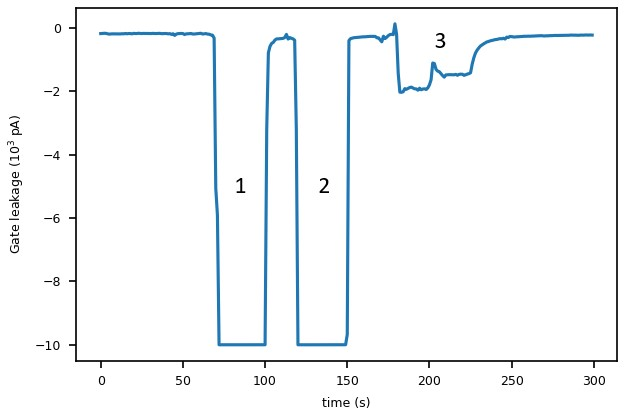
\includegraphics[width=\textwidth]{Pic/Gate_leak.jpg}
         \caption{}
         \label{}
     \end{subfigure}
     \hfill
     \begin{subfigure}[b]{0.4\textwidth}
         \centering
         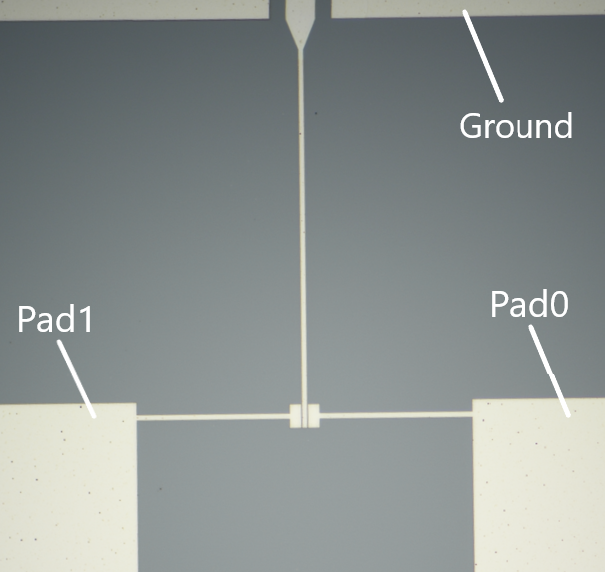
\includegraphics[width=\textwidth]{Pic/GateTest_overview.png}
         \caption{}
         \label{}
     \end{subfigure}
    \caption{The gate leakage measurement on the chip. The dip 1 and 2 indicate the grounding of contact pads 0 and 1, and 3 indicate the grounding ground.}
    \label{fig:my_label}
\end{figure}
One solution to this issue is adding an ALD layer ($\text{HfO}_2$) on top of the bottom gate to reduce the distance between the source of the electric field and the Josephson junction. In this case, the junctions can be pinched off more frequently. The limitation is that the superconductor coated on the nanowire will directly touch the ALD layer, which might introduce extra noise channels, such as a two-level system on the ALD surface, to the qubit. Also, the nanowires are not guaranteed to be pinched off before leakage. 
\begin{figure}[h!]
    \centering
    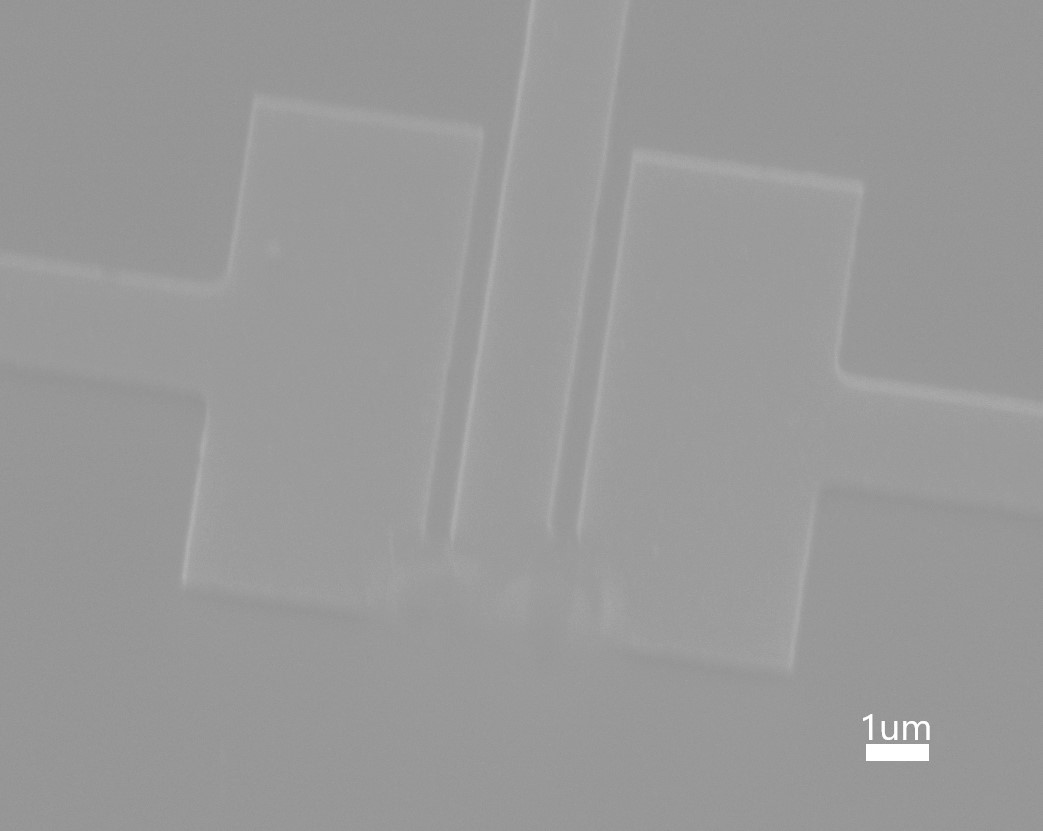
\includegraphics[width=0.6\textwidth]{Pic/GateTest.jpg}
    \caption{The 'explosion' happens after a huge leakage through the substrate. The SEM image tells us that the electric field is concentrated at the end of the gate line.}
    \label{fig:my_label}
\end{figure}

Changing Silicon to a Sapphire substrate is another solution to solve this problem by slightly adjusting the design of the qubit to have impedance matching. Sapphire has a lower dielectric constant, which can endure higher gate voltage before leakage. 

Experimentally we find that Sapphire indeed increases the leakage tolerance. Thus we can pinch off the nanowires more frequently. However, the leakage will occasionally happen at around -5V, possibly because of the short distance between the gate and the nanowire when there is an ALD layer. This is easily solved if we use the half-etched gate on an Aluminum-based chip but is hard to solve with a Tantalum-based chip due to the aggressive wet-etch recipe. Nonetheless, the dry-etch technique can possibly solve this issue and endows higher resolution, more uniform edges to the control line. We will consider doing dry-etch in the future.

\subsection{Four-terminal measurement on Tantalum nanowires}

The VLS shadowed Aluminum nanowires have been investigated thoroughly on DC measurement\cite{RN38}. Therefore our main focus in this thesis is to measure the transport properties of the new growth InAs-Ta shadow nanowires QDev 1226. The nanowires' junctions are shadowed by the nanowires with diverse shapes in front of them. Therefore the junctions behave differently due to the distribution of tantalum on semiconductors. 

\subsubsection{DC measurement on straight Tantalum nanowire}
\begin{figure}[h!]
    \centering
    \begin{subfigure}[b]{0.48\textwidth}
         \centering
         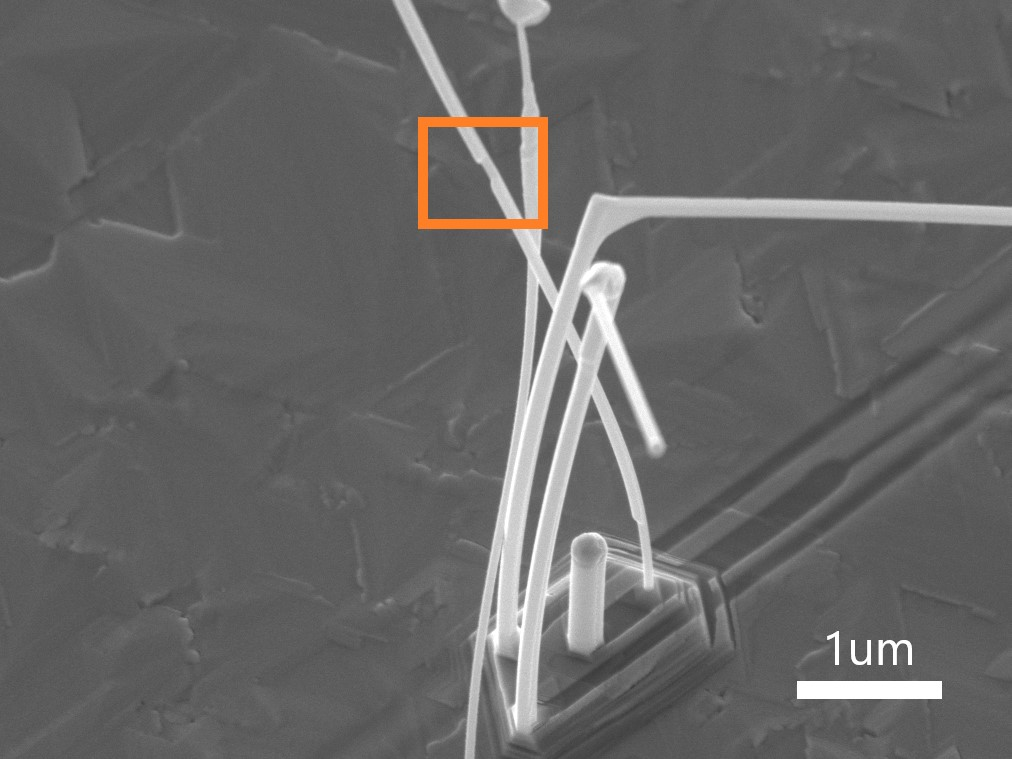
\includegraphics[width=\textwidth]{Pic/NW2_SEM_zero.jpg}
         \caption{}
         \label{}
     \end{subfigure}
     \hfill
     \begin{subfigure}[b]{0.48\textwidth}
         \centering
         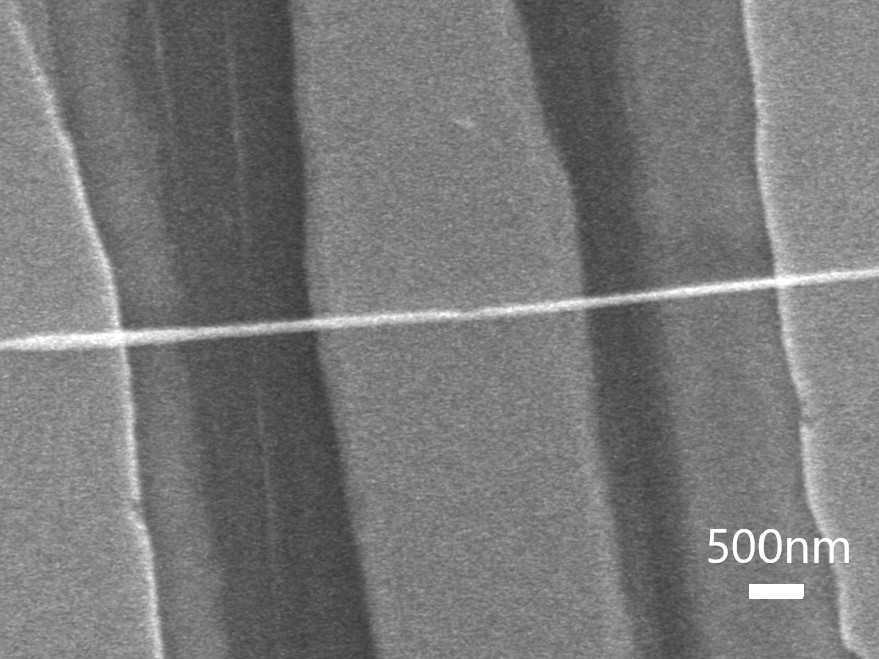
\includegraphics[width=\textwidth]{Pic/NW2_SEM_first.jpg}
         \caption{}
         \label{}
     \end{subfigure}
     \caption{The SEM pictures (a) before transferring onto the chip. The junction is highlighted in the box. (b) After transferring but before the contacts deposition and measurement. The resolution is very low because we want to reduce the SEM time, thus the charge poisoning on the junction.}
    \label{Ibiasnw2}
\end{figure}
\begin{figure}[h!]
    \centering
    \begin{subfigure}[b]{0.48\textwidth}
         \centering
         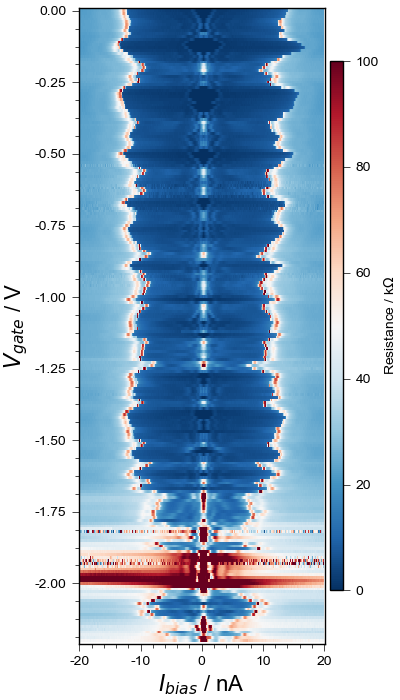
\includegraphics[width=\textwidth]{Pic/NW2_finerscan_currentbias.png}
         \caption{}
         \label{}
     \end{subfigure}
     \hfill
     \begin{subfigure}[b]{0.48\textwidth}
         \centering
         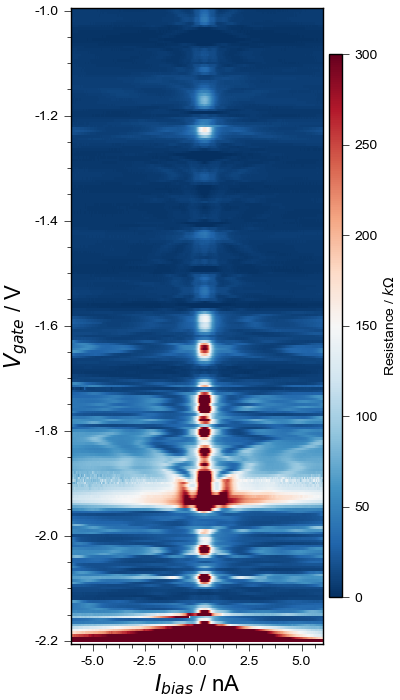
\includegraphics[width=\textwidth]{Pic/NW2_finerscan_currentbias_0.png}
         \caption{}
         \label{}
     \end{subfigure}
     \caption{Current bias measurement of Tantalum nanowire in dilution fridge, with differential resistance $dV/dI$. The DC bias current sweeps from left to right. (a) The overall current bias measurement until the nanowires are saturated. (b) Zoom in scan inside the supercurrent regime.}
    \label{Ibiasnw2}
\end{figure}
\begin{figure}[h!]
    \centering
    \begin{subfigure}[b]{0.48\textwidth}
         \centering
         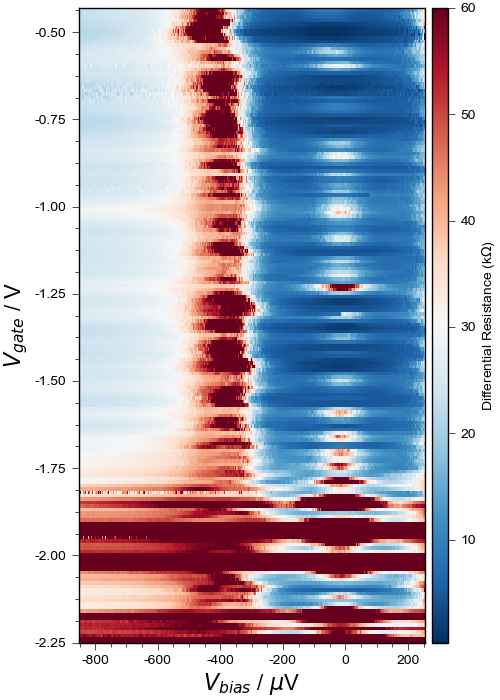
\includegraphics[width=\textwidth]{Pic/NW2_Vbias.png}
         \caption{}
         \label{}
     \end{subfigure}
     \hfill
     \begin{subfigure}[b]{0.48\textwidth}
         \centering
         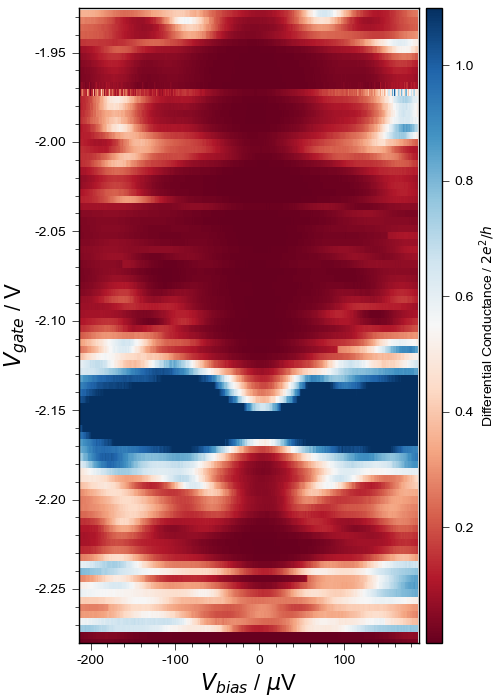
\includegraphics[width=\textwidth]{Pic/NW2_Vbias_zoom.png}
         \caption{}
         \label{}
     \end{subfigure}
     \caption{The voltage bias measurement plotted in differential resistance and conductance respectively on the straight nanowire. (a) The overall voltage bias scan until normal resistance shows up on the device. We can see a lot of recurring resistance fluctuation and dot-like events inside the superconducting gap. The measurement is asymmetric due to the large offset while doing the voltage bias measurement. (b) The zoom-in voltage bias scan inside the superconducting gap at high gate voltage near pinch off. No supercurrent occurs, and the dot-like oscillation fills the subgap.}
    \label{Ibiasnw2}
\end{figure}
In current bias measurement, we seek the critical current $I_C$ of the Josephson junction. It is a crucial parameter in calculating the Josephson energy, then the approximate operating frequency of qubit. The applied gate voltage should tune the critical current. Combining Eq \ref{JJenergy} and with the equation:
\begin{equation}
    f_{01} \approx (\sqrt{8E_CE_J}) / h
\end{equation}
, we can know that to modulate the qubit frequency in 4-6 GHz, we need to tune down the gate so that the $I_C$ can reach down to 20-45 nA. 

This nanowire has a Josephson junction of 150 - 200 nm in length. We do a quick SEM check before contact deposition to ensure the junction is on top of the gate, but we can't precisely measure the length of the junction since we only get a low-resolution image.

From the figure, we can clearly see the critical current is tuned by applying a gate voltage, and its value varies around 20-45 nA. There are complicated conductance fluctuations inside the critical current regime, indicating that Andreev reflections are perturbed by some states that occur inside the Josephson junction. The junction becomes highly resistive when $V_{gate} < -2.3 V$, indicating it can enter a tunneling regime with only a few conducting channels inside the junction that provide electrons and holes. 

In order to further understand the transportation property of the junction, we use voltage bias measurement to find out the situation inside the superconducting gap after the resistance of the junction is higher than several thousand Ohms. Otherwise, we measure in an equivalent current bias (explain later). The voltage bias data shows the approximate induced superconducting gap $\Delta^*$ of this nanowire is around 150 $\mu eV$ (estimate at $V_{gate} = 2.10 V$). The measurement data still looks noisy even if the junction is close to pinch-off. 

\begin{figure}[h!]
    \centering
    \begin{subfigure}[b]{0.54\textwidth}
         \centering
         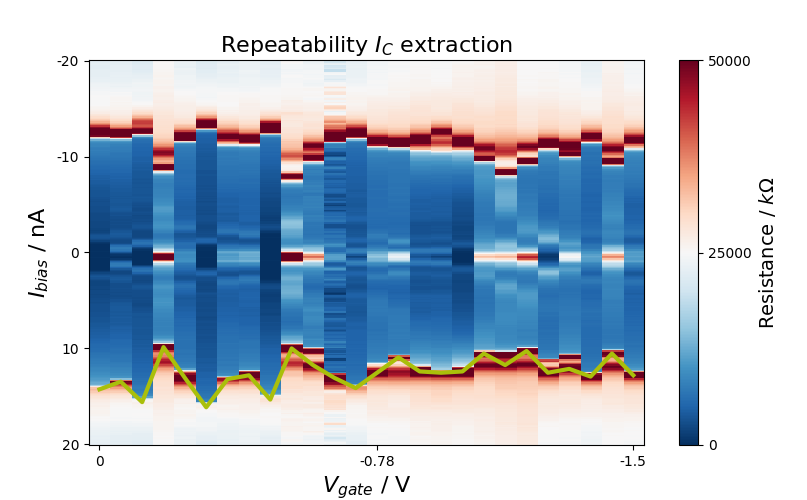
\includegraphics[width=\textwidth]{Pic/Ic_rep_extract.png}
         \caption{}
         \label{}
     \end{subfigure}
     \hfill
     \begin{subfigure}[b]{0.44\textwidth}
         \centering
         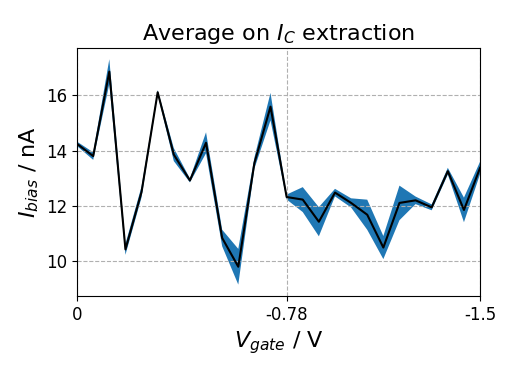
\includegraphics[width=\textwidth]{Pic/Ic_average.png}
         \caption{}
         \label{}
     \end{subfigure}
    \caption{(a) One of the ten repeat current bias measurement data. The critical current is extracted from the plot, with the bias current sweeping from negative to positive. (b) The critical current average plot for ten repetitions.}
    \label{TaNWonchip2}
\end{figure}
Two other important factors for making a good transmon qubit are the repeatability and stability of a nanowire. The former indicates the accuracy of recurrence of the critical current, hence qubit frequency, in certain gate voltage. The more accurate we can repeat the critical current, the easier we can improve our qubit gate manipulation in the future. The lateral one tells us the variation of the qubit frequency at fixed gate voltage in the unit of time. In the implementation of any time domain measurement, including gate operation and time domain measurement in a qubit, we want the qubit frequency to be stable forever.


The repeatability of the nanowire is relatively high, with almost the same change in amplitude regarding the gate voltage ten times. Moreover, the stability measurement in 3 hours demonstrates a robust Josephson junction against charge jump for a reasonably long time.

\begin{figure}[h!]
    \centering
    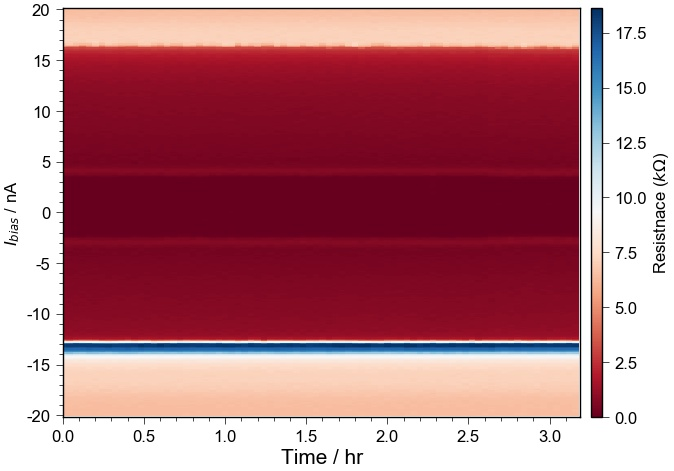
\includegraphics[width=0.7\textwidth]{Pic/Ibias_sta.jpg}
    \caption{Stability measurement on the tantalum nanowires. The current sweep is from negative to positive.}
    \label{fig:my_label}
\end{figure}


This nanowire is promising since both stability and repeatability show good robustness on the shadow Josephson junction. Nevertheless, the quantum dot-like behavior makes the wires unsuitable for gate-tunable Josephson junction in the qubit island on gatemon. It provides additional states that will break the coherence of particles inside the junction. 
\begin{figure}[h!]
    \centering
    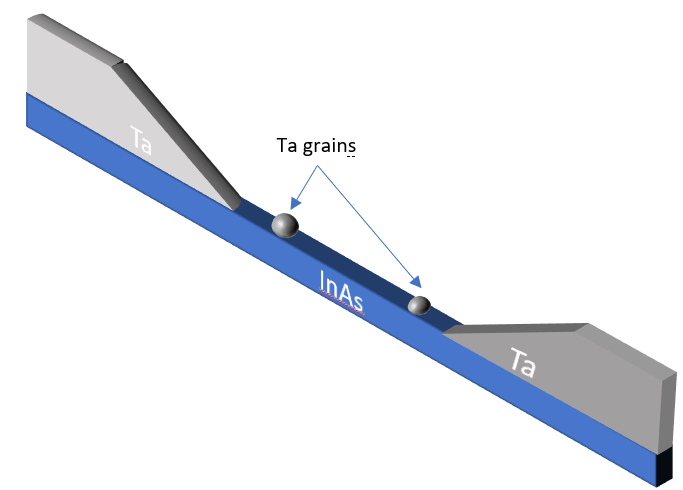
\includegraphics[width=0.6\textwidth]{Pic/TaGrain.png}
    \caption{The formation of grain on the junction can potentially provide extra states inside the superconducting gap.}
    \label{fig:my_label}
\end{figure}
The emergence of this behavior has many potential hypotheses. One possible reason for this phenomenon's formation is the unintentional tantalum grain growth on the junction. While depositing the metal on the nanowire, the atoms will diffuse into the junction and start to form grains on it. Intuitively we can imagine that the grains break the coherence of electrons and holes that participated in Andreev reflections and also reduce the mean free path of them. From an energy level perspective, these grains will provide extra energy levels inside the superconducting gap, interrupt Andreev reflections and thus introduce resistance when there is a small amount of conducting channels inside the junction. 


Further proof of whether the Tantalum nanowires have actual sub-gap states that prevent clean Andreev Reflections, hence supercurrent, from appearing, we need to find more wires to measure.

\subsubsection{DC measurement on straight nanowire 2}
According to the SEM image, the second nanowire has a 200 nm Josephson junction (Fig \ref{NW2}). 
\begin{figure}[h!]
    \centering
    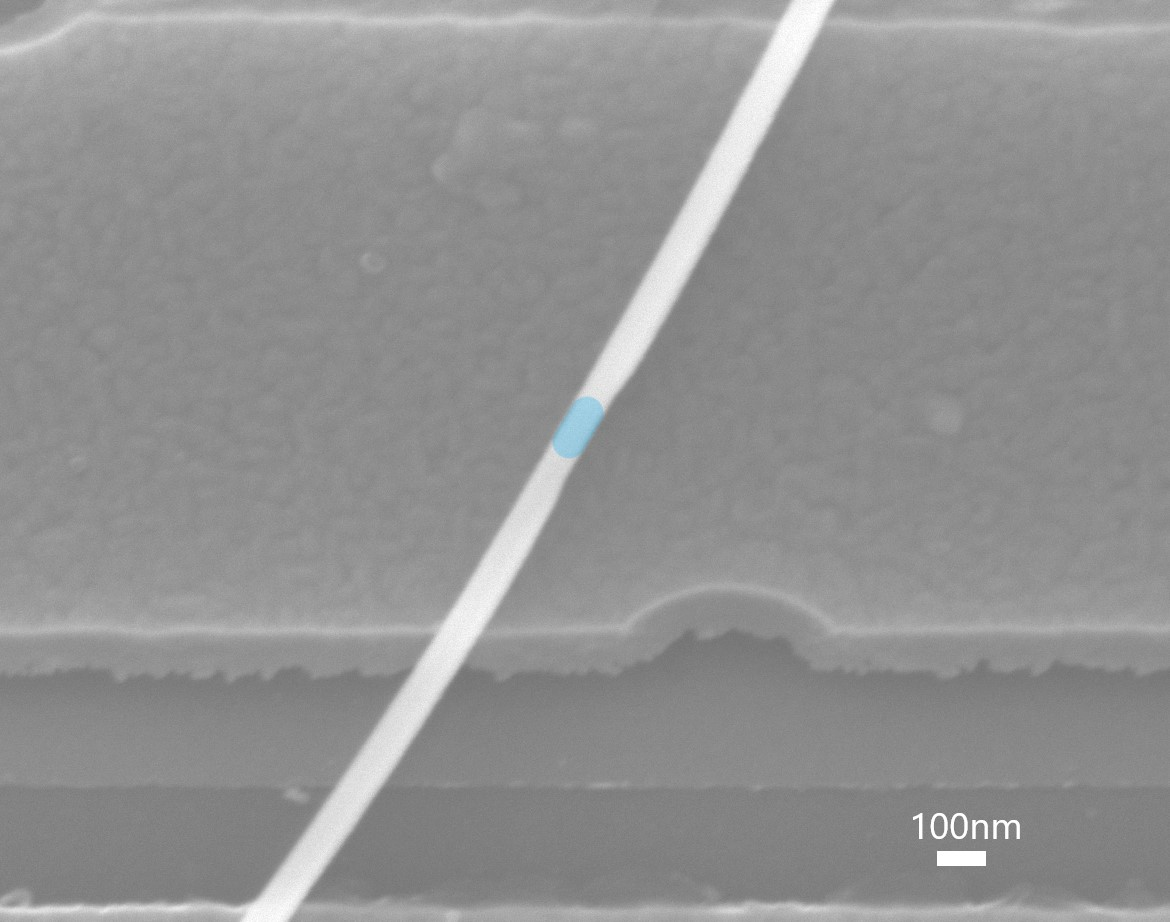
\includegraphics[width=0.6\textwidth]{Pic/D3.jpg}
    \caption{The nanowire overview in the SEM after transferring. The blue strip indicates the location of the junction, but not the length of it, since the tantalum-InAs interface has a large slope. }
    \label{NW2}
\end{figure}

After cooling down to the base temperature (25 mK) in the dilution fridge, we first try to sweep the gate without bias current.
\begin{figure}[h!]
    \centering
    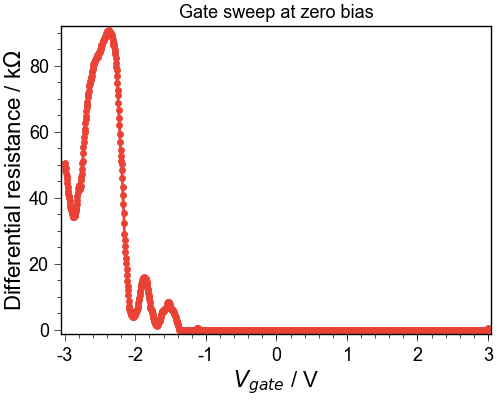
\includegraphics[width=0.7\textwidth]{Pic/D3_gatesweep.png}
    \caption{The gate sweep on the nanowire at zero DC bias current, with AC current 5 nA.}
    \label{fig:my_label}
\end{figure}

It is clear that the supercurrent exists and no dot-like behaviors before -1.4 V. The resistance increases when the gate voltage is more significant, and it shows some oscillations as the voltage changes.

\begin{figure}[h!]
    \centering
    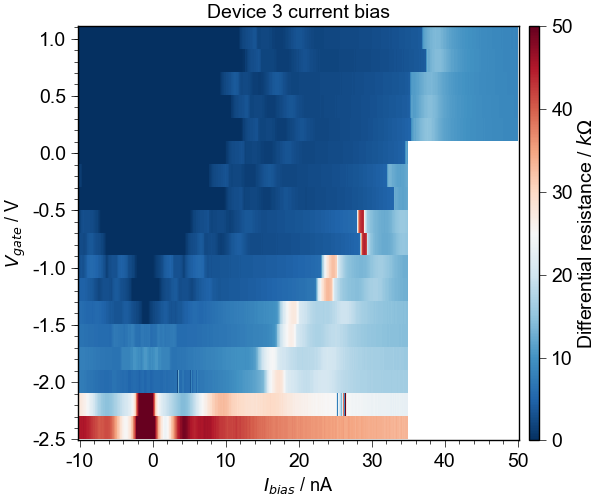
\includegraphics[width=0.8\textwidth]{Pic/D3Ibias.png}
    \caption{The current bias measurement in the unit of kOhm. The junction is partly superconducting inside the critical current regime, except for the finite resistance at the 'sleeve'.}
    \label{D3 current bias}
\end{figure}

The current bias sweeps from -10 nA to 50 nA. We can observe some resistance at a relatively large bias current before reaching the critical current, which is tuned along with the critical current. An explanation for this is the existence of different transmission rates in conductance channels. The Andreev reflections contain multiple channels, and their combination forms the supercurrent. Hence, if there are three types of Andreev reflections with different transmission rates and critical currents, the current bias map might show three boundaries (As shown in Figure \ref{D3 current bias}), and all are gate tunable. The blank part is due to the reduction of the sweeping range to 35 nA.

In voltage bias measurement, we can tune the junction into a tunneling regime, which almost eliminates Andreev reflections and leaves many specular reflections at the interface. We now get a highly resistive junction, and the voltage output from the DC source is mostly dropped on the junction. Therefore, we can estimate the induced superconducting gap from the measured $4\Delta^*$ of the junction. In Fig \ref{D3Vbias}, the line cut at $V_g = -2.4 V$ shows that the induced superconducting gap $\Delta^* \approx 110\mu eV$, which is lower than the superconducting gap of bulk tantalum (crystalline) $\alpha-$phase tantalum $\Delta_\alpha \approx 1.4 meV$ and amorphous $\beta-$phase tantalum $\Delta_\alpha \approx 300 \mu eV$. 
\begin{figure}[h!]
    \centering
    \begin{subfigure}[b]{0.75\textwidth}
            \centering
            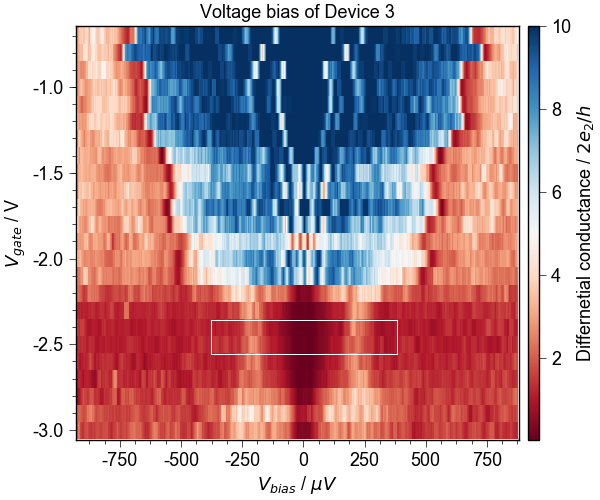
\includegraphics[width=\linewidth]{Pic/D3_Vbias.png}
            \caption{}
            \label{fig:my_label}
     \end{subfigure}
     \hfill
     \begin{subfigure}[b]{0.75\textwidth}
            \centering
            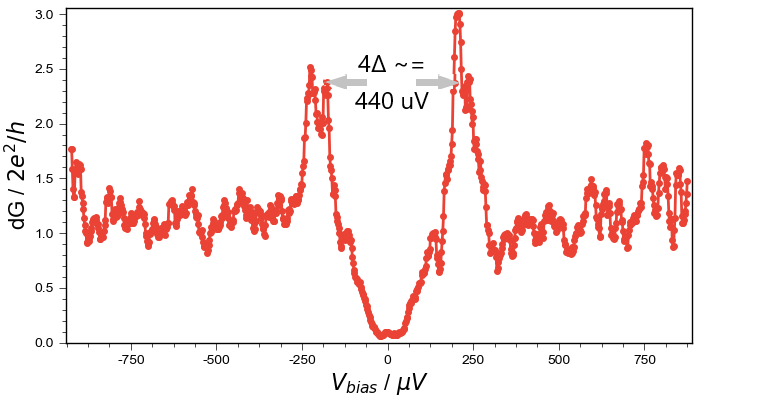
\includegraphics[width=\linewidth]{Pic/D3Vbiaslinecut.png} 
            \caption{}
            \label{fig:my_label}
     \end{subfigure}
    \caption{(a) The voltage bias measurement on the nanowire. The wire can enter the tunneling regime, but the signal is pretty noisy. (b) The line cut is at gate voltage -2.4 V. The measured superconducting gap is about 110 $\mu V$, comparable to Damon's tantalum wire \cite{RN37}.}
    \label{D3Vbias}
    \end{figure}
    
\clearpage
\subsubsection{DC measurement on kinky shadow nanowire}

\begin{figure}[h!]
    \centering
    \begin{subfigure}[b]{0.48\textwidth}
         \centering
         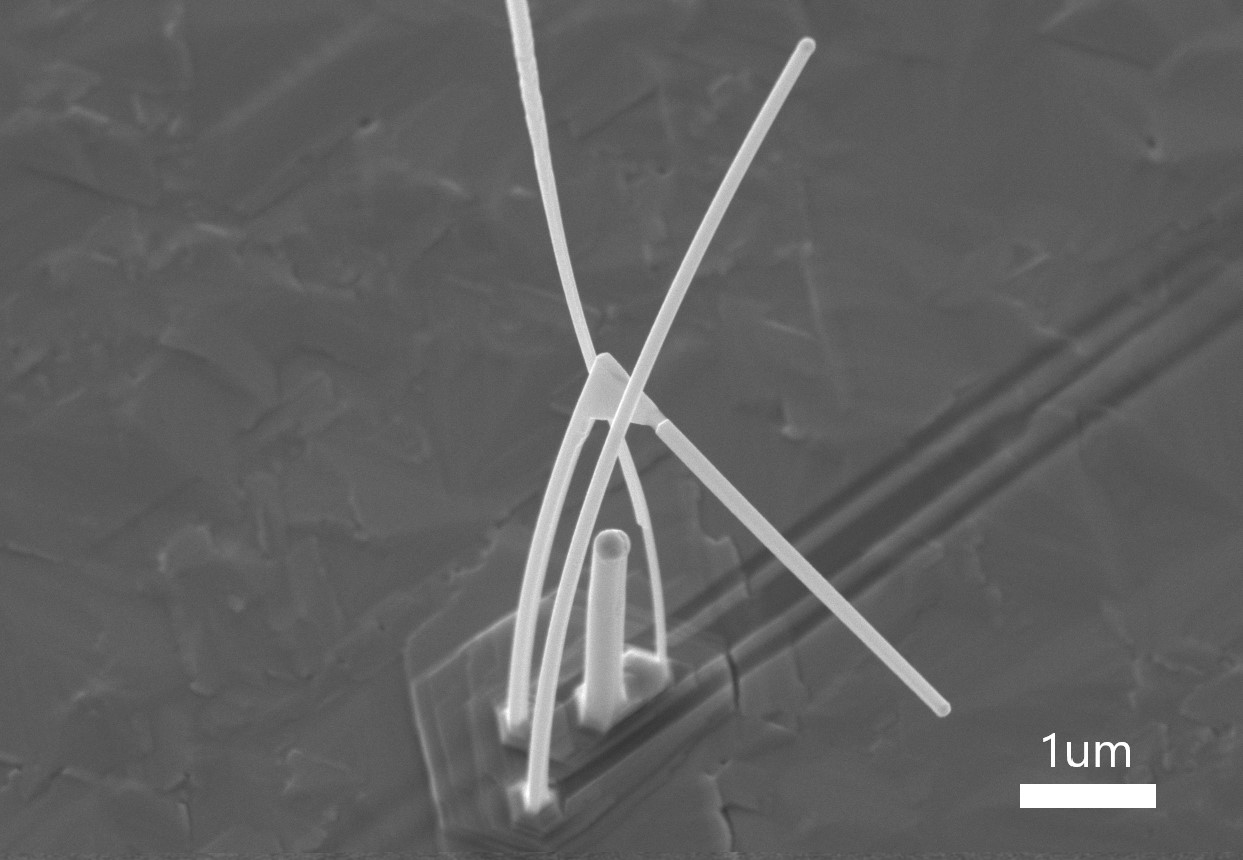
\includegraphics[width=\textwidth]{Pic/Kinkywire_SEM.jpg}
         \caption{}
         \label{}
     \end{subfigure}
     \hfill
     \begin{subfigure}[b]{0.47\textwidth}
         \centering
         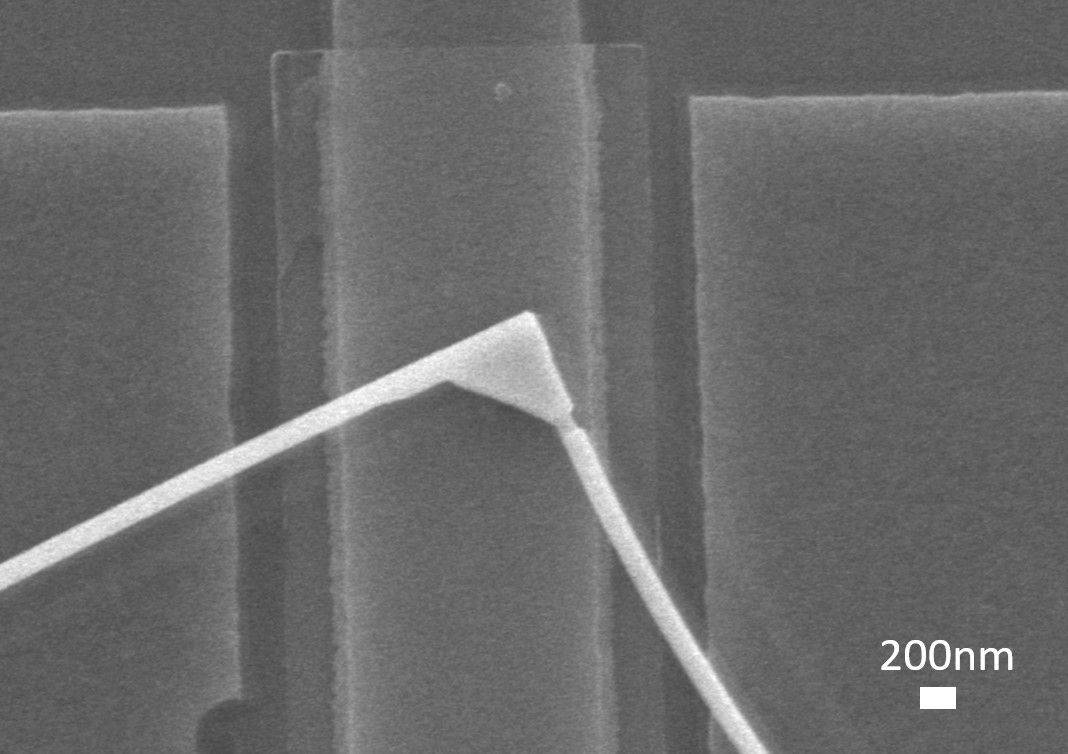
\includegraphics[width=\textwidth]{Pic/Kinkywire_SEM_0.jpg}
         \caption{}
         \label{}
     \end{subfigure}
     \caption{The kinky wire and its SEM picture on the ALD gate. Notice that the junction is around 100-150 nm.}
    \label{KinkywireSEM}
\end{figure}

The Kinky wire with shadow junction is found with luck, and its tantalum coat looks homogeneous. The S-N interfaces are spotless and clear, which may give us cleaner data than previous nanowires. Therefore it is worth to try measuring it and knowing how it behaves.

\begin{figure}[h!]
    \centering
    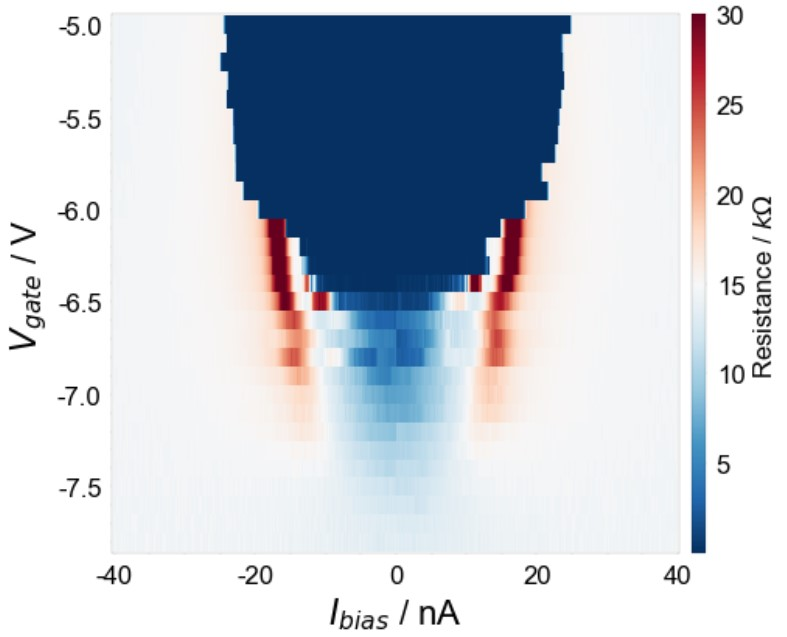
\includegraphics [width=0.7\linewidth]{Pic/DC2_NW7_Ibias_R.jpg}
    \caption{Current bias measurement of kinky wire. The sweeping is from 0 to both sides to get a critical current. The superconducting regime starts to be vague after -6.5V due to the gate leakage.}
    \label{IbiasKink}
\end{figure}

In current bias measurement, the superconducting regime of the nanowire is clean and genuinely superconducting (for the random measured phase on voltage drop to prove further that this is true supercurrent). Meanwhile, the critical current is easily turned down to 20 nA without gate leakage. This is already the optimal operating regime for gatemon. The lack of features inside the critical current area also is a good sign for having a flawless junction. However, the gate starts to leak when the gate voltage is at -6.5 V, which injects more than 1 nA current through the junction. This causes vagueness in the data and eventually vanishing of the supercurrent. The problem prevents the nanowire from entering the tunneling regime, and thus we can't measure the induced superconducting gap of this nanowire.

Since we can't tune the nanowire into the tunneling regime, and the resistance of the nanowire at zero bias is still low, the voltage bias measurement is now equivalent current bias measurement. This is because the line resistance of the fridge along the DC loom is around 3000 $\Omega$. Unless we can tune the resistance of the nanowire at zero DC bias to higher, the significant voltage drop will still be on the coaxial line, and no valid superconducting gap is shown. 

\begin{figure}
    \centering
    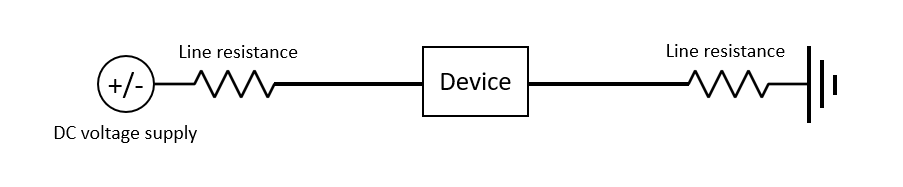
\includegraphics[width=\textwidth]{Pic/lineR.png}
    \caption{The illustration of the line resistance in the fridge. While in voltage bias measurement, we need to tune the device to high resistance. Otherwise, it is an equivalent current bias measurement.}
    \label{fig:my_label}
\end{figure}

There is yet no MARs sign in the measurements in both current and voltage, probably because we are not close to the tunneling regime of the nanowire. 

\begin{figure}[h!]
    \centering
    \begin{subfigure}[b]{0.45\textwidth}
         \centering
         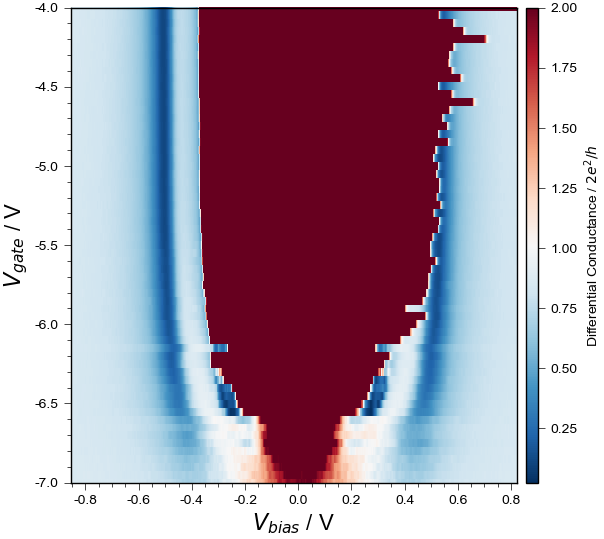
\includegraphics[width=1.1\textwidth]{Pic/KinkyVbiasCon.png}
         \caption{}
         \label{}
     \end{subfigure}
     \hfill
     \begin{subfigure}[b]{0.5\textwidth}
         \centering
         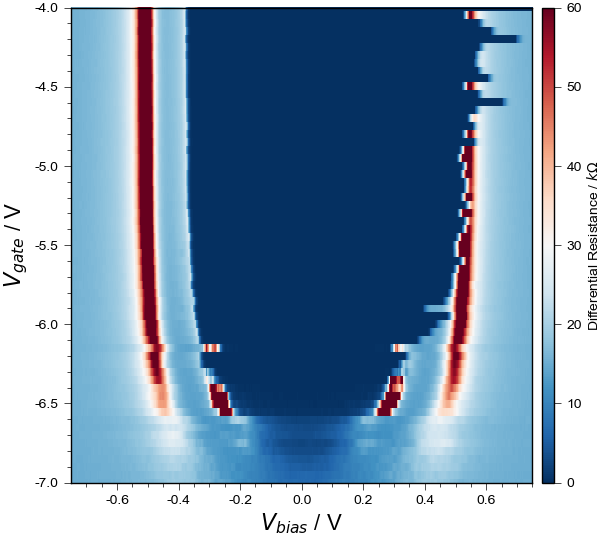
\includegraphics[width=\textwidth]{Pic/KinkyVbiasRes.png}
         \caption{}
         \label{}
     \end{subfigure}
    \caption{The voltage bias measurement plotted in (a) differential conductance and (b) differential resistance. Since the resistance is still low at zero bias, the voltage bias measurement is not valid because the voltage will drop on the coaxial line}
    \label{VbiasMSMT}
\end{figure}


